%%
%% This is file `sample-sigconf.tex',
%% generated with the docstrip utility.
%%
%% The original source files were:
%%
%% samples.dtx  (with options: `sigconf')
%% 
%% IMPORTANT NOTICE:
%% 
%% For the copyright see the source file.
%% 
%% Any modified versions of this file must be renamed
%% with new filenames distinct from sample-sigconf.tex.
%% 
%% For distribution of the original source see the terms
%% for copying and modification in the file samples.dtx.
%% 
%% This generated file may be distributed as long as the
%% original source files, as listed above, are part of the
%% same distribution. (The sources need not necessarily be
%% in the same archive or directory.)
%%
%% The first command in your LaTeX source must be the \documentclass command.




\documentclass[sigconf]{acmart}
\acmConference[Iowa State University - COMS 574 Draft Report]{574 Report}{April, 2020}{Ames, IA}
\usepackage{mathtools}
\usepackage{listings}
\usepackage{natbib}
\usepackage{hyperref}
\usepackage{url}
\usepackage{times}
\usepackage{helvet}
\usepackage{courier}
\usepackage{graphicx}
\usepackage{array}% http://ctan.org/pkg/array
\usepackage{subcaption}
\usepackage{cleveref}
\captionsetup[subfigure]{subrefformat=simple,labelformat=simple}
\renewcommand\thesubfigure{(\alph{subfigure})}
\usepackage{multirow}
\usepackage{array}
\usepackage{xcolor}
\usepackage{authblk}

\newcolumntype{L}{>{\centering\arraybackslash}m{7cm}}
\newcolumntype{Q}{>{\centering\arraybackslash}m{5
cm}}
\lstset
{ %Formatting for code in appendix
    language=Java,
    frame=single,
    morekeywords={?},
    basicstyle=\footnotesize,
    numbers=left,
    stepnumber=1,
    showstringspaces=false,
    tabsize=1,
    breaklines=true,
    breakatwhitespace=false,
    moredelim=**[is][\color{red}]{@}{@},
    moredelim=**[is][\color{blue}]{^}{^},
    commentstyle=\itshape\color{green!40!black}\bfseries,
}

%%
%% \BibTeX command to typeset BibTeX logo in the docs
\AtBeginDocument{%
  \providecommand\BibTeX{{%
    \normalfont B\kern-0.5em{\scshape i\kern-0.25em b}\kern-0.8em\TeX}}}



\begin{document}
\title[CodeBasedStarPrediction]{Code based Github Projects Popularity Prediction}
\author[1]{Hung Phan}
\affil[1]{Department of Mathematics, University X}




%%
%% The abstract is a short summary of the work to be presented in the
%% article.
\begin{abstract}
\end{abstract}

%%
%% The code below is generated by the tool at http://dl.acm.org/ccs.cfm.
%% Please copy and paste the code instead of the example below.
%%

%%
%% Keywords. The author(s) should pick words that accurately describe
%% the work being presented. Separate the keywords with commas.
\keywords{Machine Learning Regression, Machine Learning Classification}



%%
%% This command processes the author and affiliation and title
%% information and builds the first part of the formatted document.
\maketitle

\section{Introduction}
Deep Learning (DL) has been applied in different Software Engineering (SE) researches and problems\cite{001,002,003}. It can contribute to all stages of software development life cycle, from requirements extraction, design, implementation to maintenance \cite{001}. Since DL was vastly applied earlier in Natural Language Processing (NLP), a popular trend of applying DL in SE is to consider the input of SE problems as different types of documentation similar to NLP input. According to \cite{003}, there are 3 main types of documentation: Natural Language (NL), Software Documentation (SD) and Programming Language (PL). Based on the requirement of each tasks, the output of research works that used these types of documentation as input is varied by different types of code tokens. For the research works that used NL as input, they tend to find the element of code environment that satisfied the description in NL, which they applied for code search \cite{004,005} and code synthesis \cite{006}. SD is special type of documentation written in NL but contains information about description of the Application Programming Interfaces (APIs) of different programming languages. There is a work in the literature on representing APIs as vector from SD \cite{007}. For the research works used PL as input, they used deep learning translation between PLs \cite{009} and code suggestion \cite{008}.

The output of DL researches in SE problems can not only be the source code or code tokens, but also could be the information from SDs and NLs.  Different applications are proposed to translate between each types of documentations using Machine Learning (ML). There are works on generating SD as pseudo-code from code using DL and ML \cite{010,011}, or generating documentation from API specifications \cite{012}, or generating commit messages in NL \cite{013}. Neural Machine Translation (NMT), which is a technique relied on advantages of DL, can be assumed as the best translation engine for SE. The ability of NMT relies on the formation on multiple layers of neural network to capture more information for the translation of each elements in the source language \cite{014}. Besides, along with text sequence, NMT can be applicable on a different data structure such as graph or tree, which is suitable for the representation of code \cite{015}. Another advantage of NMT is the performance for inferring the results, which is usually outperform earlier Machine Translation techniques \cite{014}.

Before the era of NMT, Statistical Machine Translation (SMT) \cite{016} was the most popular technique for solving SE problems which relied on MT approaches. With the idea of extending the original Bayes rule \cite{017}, SMT provides the ability of learning the context in Natural Language for translation between popular languages. Since the source code also embed information of NL \cite{018}, SMT is successfully be applicable of SE problems as translation between versions of Python \cite{019} and between different PLs \cite{020}. However, compared to newer trends of translation engines such as NMT, SMT reveals 2 drawbacks. First, it cannot learn information from long sequence of text. An implementation tool of SMT, Phrasal \cite{021} can only process the phrase with maximum length of 7. Secondly, the training and testing time of SMT become worse with large training data and increases exponentially \cite{022}. For these reasons, NMT has replaced SMT in SE problems \cite{010,011}.

Although having many advantages, NMT itself contains some challenges which also appear in researches of different areas along with SE. \cite{024,023} mention about an important problem of NMT compared to SMT as rare words problems in NLP. Current popular NMT engines, OpenNMT \cite{025} or Google NMT \cite{026}, cannot handle large size vocabulary with more than 100000 words. To optimize the problem, researchers considered rare words as Unknown words which their translated results are not counted to the final results. This fact caused NMT performs poorly when rare/unknown words are frequent in the corpus \cite{024}. In SE researches, the problem of Type Inference using MT shows that SMT model provided by \cite{028} has a significant higher accuracy compared to the original NMT approach in \cite{027}. Similarly, for natural language diacritic restoration, \cite{029} shows that SMT outperforms NMT.  \cite{026,027,028} have the same characteristics of parallel corpus, i.e., the length of source and target pairs are equal and the order of the source and target words are consistent with each other. This leads us to an assumption that if the parallel corpus for training MT has these characteristics, it will affect the accuracy of NMT. In summary, NMT tends to have lower accuracy than SMT due to the methodology of NMT that didn't support the rare words translation and the characteristics of parallel corpus. 

In this work, we further investigate the efficiency of NMT vs. SMT in a new research problem that has similar characteristics of parallel corpus as \cite{026,027,028}. Instead of focusing on only limited types of tokens in code environment, our problem provide a solution to help developers get the code of all types of code tokens based on its first letters in the form of abbreviation/prefix of tokens. To implement the solution for this problem, we build two spaces of abbreviations of code tokens as source language and code tokens as target language. Then, we implement two machine translation models, Neural Machine Translation and Statistical Machine Translation to learn the mapping from prefixes to code tokens for code suggestion. We also analyze the affect of unknown tokens along with the accuracy on each types of tokens. By the evaluation, we show that SMT outperforms the original NMT. We called our approach PrefixMapping and analyze the effective translation on three types of documentation: NL, SD and PL. Overall, this paper provides the following contributions:

\begin{enumerate}
\item Proposing the translation based engine for code completion from first letters of tokens.
\item Providing algorithms for extracting parallel corpus of prefixes and tokens in 3 types of documentation used in NLP and SE.
\item Implementing and Optimizing Statistical Machine Translation for PrefixMapping.
\item Implementing and Optimizing Neural Machine Translation for PrefixMapping.
\item Analyzing the accuracy of NMT compared to SMT along with accuracy depending on each types of code tokens.
\end{enumerate}

The structure of the paper is provided as follow. In the next section, we will describe about our research problem. In this section, we will define important concepts we use for abbreviations, algorithms for data collection, and the overview architecture of the system. The core engines of translation, NMT and SMT, along with their optimization for this problem is described in the third section. In the evaluation, we will provide the accuracy and head-to-head comparison between NMT and SMT in 3 types of documentation. We published our data and code at \cite{053}.






\section{Prefix Resolution}
\cite{027,028} provide a translation approach considered the source side language as partial class name (PCN) and the target language as Fully Qualified Name (FQN) of APIs. \cite{029} treated the source language as a word without diacritic information and the target language as a word with diacritic information. In other words, both of these research works build a parallel corpus with the same length of source sequence and target sequence to each pair. The orders for source and for target sequences are also consistent. In summary, the problem of translation in \cite{027,028,029} has the common in characteristics of parallel corpus.

In our work, we design an inferring system based on translation inspiring from 
\cite{028}. While \cite{028} focuses on the class name of APIs as the source language, we provide our source language as types of abbreviation for each words in a documentation corpus. Depending on different level of abbreviation, we build multiple translation models based on different length of the first letters for each words in parallel corpus. We have some definitions of elements in our context of translation problem. 
\begin{definition}
    \label{def001}
  \textbf{Prefix}: Given a word or code token, the prefix of a word is a word that combined by the set of first letters which developer can input to the code editor. 
\end{definition}
\begin{definition}
\label{def002}
  \textbf{n-letter(s) Prefix}: The n-letter prefix of a word/ code token is the prefix that has length of n letter. 
\end{definition}

We see examples of these definition in PL in the Listing \ref{example001}. This code snippet is the method declaration of event function fireQueueStateChanged() from \cite{030}. This function is to handle the event for Android version of Vodaphone devices. From this function, we see that there are many kinds of code tokens, including program keywords, class name, method name and variable names. Look at the token notifyOfItemInRequestQueue() as an example. In this token, its 1-letter prefix is \texttt{n}. Its 3-letters prefix is \texttt{not} and 9-levels prefix is \texttt{notifyOfI}. We provide a code suggestion that allows developers to write multiple prefixes at 1 level, 3 levels and 9 levels. Then, in the next step, the machine translation will translate from the area of n-levels prefixes to suggest the full tokens. We do not restrict on any kinds of code tokens. In the other words, we support suggesting tokens for all types of prefixes. 

To implement the solution, we do the following steps. First, we collect the data for software projects. Next, we extract the information from source as prefixes and target as the code tokens by the visiting code at Abstract Syntax Tree (AST) tree structure. Depending on the how many letters of the input prefix, the application will load the training models for the same letters prefixes inference. In the final step, the suggestion of code tokens from prefixes is provided. Example of tokens from source and target language at different n-letters is provided by this table:

% Please add the following required packages to your document preamble:
% \usepackage{multirow}
\begin{table}[]
\small
\label{tbl001}
\caption{Example of source target tokens for Prefix Mapping at n-letter(s) prefixes }
\begin{tabular}{|l|l|l|}
\hline
\multirow{6}{*}{Source} & 1-letter   & s ( m ) \{ L . l ( " ( ) \_ + m + " ) ;                        \\  
                & prefix  & f ( I l : m ) \{ l . n ( ) ; \} \}                       \\ \cline{2-3} 
                        & 5-letters  & synch ( mList ) \{ LogUt                                         \\  
                        & prefix & . logW ( "Requ ( ) \_list + ...                                          \\ \cline{2-3} 
                        & 9-letters  & synchroni ( mListener ) \{ LogUtils . logW       \\          
                        & prefix & ( "RequestQ ( ) \_listener + ...      \\ \hline
\multirow{2}{*}{Target}                  & Code       & synchronized ( mListeners ) \{ LogUtils . logW  \\
&   tokens   & ( "RequestQueue.notifyOfItemInRequestQueue ( )... \\
\hline
\end{tabular}
\end{table}

\\
\noindent
\begin{lstlisting}[basicstyle=\small,caption={Example of code snippet \cite{030}},label={example001}]
protected void fireQueueStateChanged() {
	synchronized (mListeners) {
		LogUtils.logW("RequestQueue. notifyOfItemInRequestQueue () listener["
				+ mListeners + "]");
		for (IQueueListener listener : @mListeners@) {
			listener. @notifyOfItemInRequestQueue@() ;
		}
	}
}
\end{lstlisting}

\subsection{Architecture Overview}
The architecture overview of our tool, PrefixMap is provided as follows. We provide a code editor that accept developers to write abbreviation of code tokens in the form of first letters. After this step, we have the input as the mix of full code tokens and prefixes. The length of prefix can be varied. Then the information of code will be parsed by an Abstract Syntax Tree (AST) Parser to collect the code to sequence of prefixes. Each prefixes of code tokens will be encoded into the sequence as the source sequence for translation. Then, the MT engines will convert the sequence of prefixes to sequence of tokens, which shows suggestions for each input prefixes. For example, \texttt{mList} and \texttt{notif} prefixes in Listing \ref{example001} will be translated to the expected tokens which are \texttt{mListeners} and method name \texttt{notifyOfItemInRequestQueue}. To be able for inference in the testing phase, we provide the training phase with the source language as prefixes and target language as code tokens from 1000 Github Corpus we collect from MSR 2013 \cite{031}.

From the architecture overview, we can see two important points we need to address compared to other neural machine translation works. First, we considered the both 2 MT engines for fixing the prefixes. We show the strength and the disadvantages of each MT models for this problem. Secondly, the PrefixMap was trained based on the parallel corpus with consistent in length of tokens and order of source and target tokens. Third, in our approach, each source tokens needs to be mapped with a target tokens, means the cases of unknown tokens will be affected since the MT cannot provide the suggestion. We will study about the affect in the Evaluation section.

\begin{figure*}
        \center{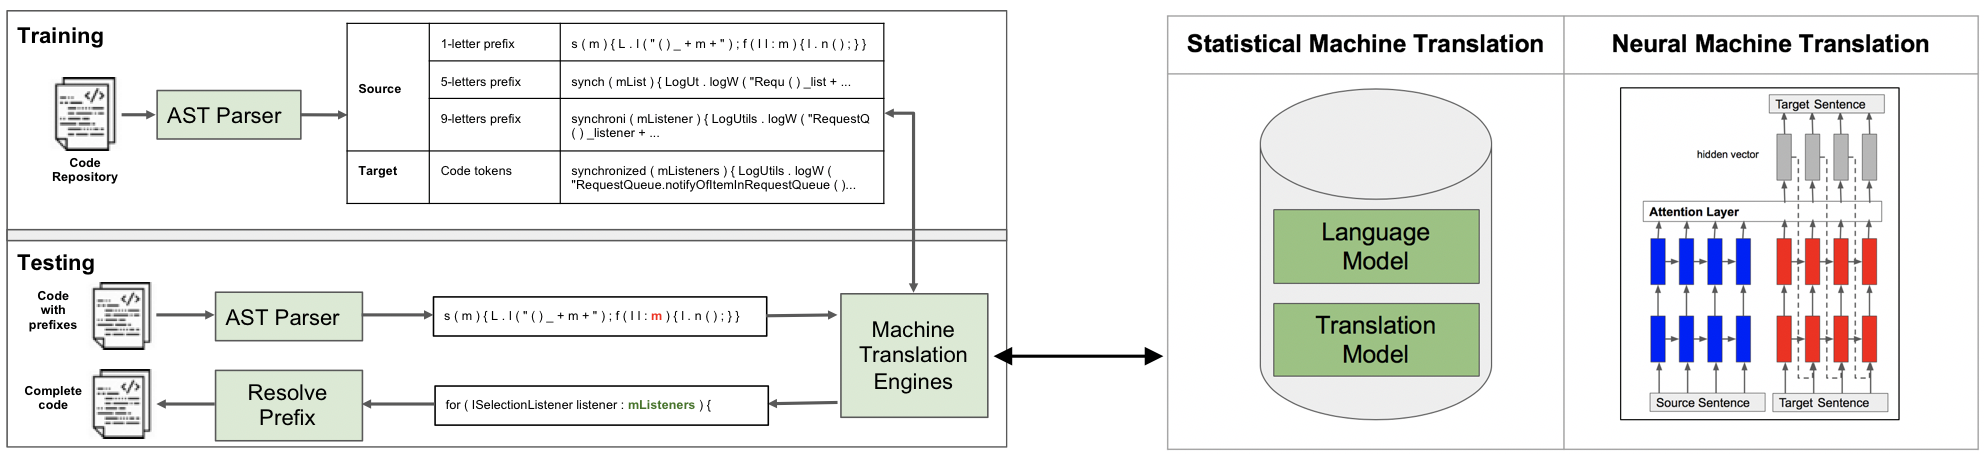
\includegraphics[width=\linewidth]
        {images/architecture.png}}
        \caption{PrefixMap Architecture Overview}
        \label{fig:mapping_expression} 
\end{figure*}

\section{Machine Translation Engines}
In this section, we discuss about the algorithm for data extraction and the algorithm for SMT and NMT.
\subsection{Data Extraction}
The algorithm of extracting source side and language side is provided in Listing \ref{algm001}. The core of implementation is done by an AST parser we extended from the source code of Eclipse JDT \cite{032}. In this parser, we enhance the default \texttt{visit()} function which accepts an ASTNode object to a new function \texttt{visitAndExtract()}. This function behaves specifically to the MethodDeclaration node and the ASTNode objects inside this MethodDeclaration. The function for other AST objects accepts the node, the level of prefixes and the pair object. For each pairs, they contain one sequence of tokens as source and one sequence of tokens as target. Inside this function, first it will extract all tokens inside the ASTNode. Next, it will extract the prefix at n-levels for each tokens by a for loop. Final, the source and target sequence are included in the a new Pair object before adding the new object to the list. The \texttt{visitAndExtract()} function for MethodDeclaration accepts a list of pairs as input. It will create a new Pair object, visiting each ASTNode objects in the sub tree of this MethodDeclaration and extract the prefixes and related code tokens in training Github projects. 
\begin{lstlisting}[basicstyle=\small,caption={Algorithm to extract the source and target sequences by ASTParser in PrefixMap},label={algm001}]
class PrefixMapVisitor extends ASTVisitor{
    ...
	void visitAndExtract(MethodDeclaration node,int level,List<Pair> list) {
	    Pair p=new Pair();
	    node.getBody().visitAndExtract(node,level,p);
	}
	...		
	void visitAndExtract(ASTNode node,int level,Pair p) {
		String[] tokens= getTokens(node);
		
		for t in tokens{
		    String sToken=getPrefix(t,level);
		    p.getSource().append(sToken);
		    p.getTarget().append(t);
        }
	}
	...
}
\end{lstlisting}
For example in Listing \ref{example001}, the algorithm Listing \ref{algm001} will visit the \texttt{fireQueueStateChanged()} MethodDeclaration to extract information all ASTNode inside this function. The information provides us the content of varies of types of ASTNode, including the MethodInvocation, for loop and inside variables and inside MethodInvocation. The target side for each tokens is actually the code content, while the source side contains the prefix of the code tokens, which can be inputted by developers in the suggestion phase. There is a corner cases that the size of the required prefix is greater than the length of the code tokens. If that case happened, the prefix will encode the information of the whole token. For instance, the token \texttt{for} has the prefix at 9-letters as \texttt{for}. In the next section, we will discuss about important elements of MT engines we used. 

\subsection{Statistical Machine Translation for Prefix Map}
Our implementation of SMT for PrefixMap is based on a well-known toolkit Phrasal \cite{021} from StanfordNLP group. We call the source sequence as \texttt{Prefixes} and the target tokens as \texttt{Codes}. We call $prefix_{i}$ as the $i^{th}$ index prefix in the source sequence and $code_{i}$ as the $i^{th}$ index token in the target sequence. The purpose of SMT, along with NMT, is to calculate probability of each prefix is translated to target token given a context of code by different machine learning directions. For SMT, this probability contains 2 elements : the Language Model (LM) and Translation Model (TM),

\textbf{Language Model}. In SMT, the LM is calculated for the target language, means the sequence of code tokens in our problem \cite{035}.  Recently, there are newer LM models that encoded neural network as mentioned in \cite{036}. In SMT, it used the statistical language model approach called n-gram. The n-gram language model will assign probability for code sequences of the whole MethodDeclaration along with the sequence of code tokens inside the body of method. In general, the most useful purpose of LM is to calculate the probability of the last word of n-gram sequence given the previous code tokens. The LM approach is also applied in building code suggestion tool from very large code database such as \cite{031} . 

Theoretically, to predict the next code tokens, the larger number of n-gram produces the better of code token suggestion. However, large n-gram will cause exponential time increasing in the performance. In practical, Phrasal restricts the maximum size of n-gram as 7. The fastest n-gram, uni-gram, is not usually used since I provide the estimation only by the number of appearance for that code tokens.  The intuition of calculating the n-gram for code tokens is estimating the probability of the current n word given n-1 words by calculating the ratio between the number of appearance of sequence of n words per the number of appearance in sequence of n words. Smoothing is the technique that the LM are required if a word appeared in the unseen context to avoid the LM to assign zero probability. In our SMT implementation, we use the Kneser-Ney smoothing method, which is proposed by KenLM \cite{034,035,037}. We have the probabilistic model $P_{LM}$ as follow:
\noindent
\begin{equation*} 
\label{eq:001}
\begin{multlined}
 P_{LM}(code_{n}|code_{1}^{n-1}) = \\ u(code_{n}|code_{1}^{n-1})+b(code_{1}^{n-1})*P_{LM}(code_{n}|code_{2}^{n-1}))
 \end{multlined}
\end{equation*}

In this formula \ref{eq:001}, the language model probability for the $n^{th}$ code token is calculated recursively by the respected probability of the $(n)^{th}$ token given (n-2) tokens. This probability has 2 other elements for normalization, called pseudo probability \texttt{u()} and backoff metric \texttt{b} \cite{037}. The recursion will stop at the unigram distribution as follow:
\noindent
\begin{equation*} 
\label{eq:002}
\begin{multlined}
 P_{LM}(code_{n}|[]) = \\ u(code_{n}|[])+b(\epsilon)*\frac{1}{|voc of tokens|})
 \end{multlined}
\end{equation*}

In formula \ref{eq:002}, \texttt{[]} is the empty sequence. the code tokens which are unseen in data will have the probability of the second operand, since \texttt{u()} is equals to Zero.Example of how LM represented in PrefixMap in line 5 example \ref{example001} is shown in \ref{tbl001}. 

\begin{table}[]

\begin{tabular}{|l|l|l|}
\hline
\textbf{n-1 gram}                               & \textbf{nth token} & \textbf{PLM} \\ \hline
\multirow{4}{*}{for ( IQueueEnqueue listener :} & list                  & 0.82         \\ \cline{2-3} 
                                                & mListeners         & 0.78         \\ \cline{2-3} 
                                                & indices              & 0.66         \\ \cline{2-3} 
                                                & ...                & ...          \\ \hline
\end{tabular}
\caption{Example of 6-gram LM probability in Listing \ref{example001} }
\label{tbl001}
\end{table}

In this example, we see that the output of $P_{LM}$ suggests the list of variables given 5 previous tokens in the 6-gram LM. It shows the most popular popular variable as the \texttt{list} variable which is the first candidate suggested by the LM. However, the inference between source and target language also depends on another probability along with the probability of the target language. We have the second element of the SMT, the translation model.

\textbf{Translation Model}. The translation model integrates the information from LM, the mapping probability of the prefixes given the code tokens (called the phrase translation probability) and the reordering score between translated phrase and input phrase. The final output of this step provided by Phrasal is a data structure called Phrase Translation Table, which contains probability for each phrase as candidate for translation. There are three stages in producing the phrase table. The first stage is word alignment, which is done by IBM model 1 by default \cite{039}. Next, the phrase pairs of source and target languages are extracted. Final, the scoring phrase pairs process is done to assign the probability to phrase table. The probability of translation from prefixes to code tokens can be provided as follow:

\begin{equation} 
\label{eq:003}
Codes_{best}=argmax_{codes}p(Prefixes|Codes) * p_{LM}(Codes)
\end{equation}
In formula \cite{039}, the phrase translation probability \texttt{p(Prefixes|Codes)} contains information about the association between source and target tokens and the probability for reordering the phrases order between source and target language. The association between the phrase of source given the phrase of target language can be scored by relative frequency of their co-occurrence in the training set \cite{039}. There are several ways for estimating the phrase translation probability. In newest version of Phrasal, it used the Log Linear method, which calculate the translation model by this formula:

\begin{equation} 
\label{eq:003}
p(x)=exp (\sum_{i=1}^{3}\lambda _{i}*h_{i}(x))
\end{equation}

In this formula, the final translation probability will depend on the exponential of three features functions and 3 hyper parameters. They are log($\theta$) as the logarithm of  relative frequency, log(d) as the log of reorder penalty, and log($P_{LM}$) as the logarithm of language model probability. The input variable x is a random variable contains information about the candiate phrases and the position of phrases in source language.

\begin{table}[]
\begin{tabular}{|l|l|l|}
\hline
\multicolumn{1}{|c|}{\textbf{source}} & \multicolumn{1}{c|}{\textbf{target}}      & \multicolumn{1}{c|}{\textbf{p(t|s)}} \\ \hline
for ( I l : m                         & for ( IQueueEnqueue listener : mListeners & 0.88                                 \\ \hline
for ( I l : m                         & for ( Index listItem : m                  & 0.62                                 \\ \hline
\end{tabular}
\caption{Phrase table result of Line 5 Listing \ref{example001} }
\label{tbl002}
\end{table}

The translation probability extracted by the phrase table after training the data of Line 5 in Listing \ref{example001} is shown in Table \ref{tbl002}. In this table, we see that the probability for the phrase contained the sequence \texttt{f ( I l :} returns the phrase that contains the correct translation result as \texttt{mListeners}.

\textbf{Optimization of SMT for PrefixMap}. Since this corpus for PrefixMap has chracteristics of consistent length and consistent order between source and target language, we alternate the original SMT model for suit with our problem. First, we create our own alignment of source and target tokens instead of using IBM Model 1. Second, with the original output from SMT, we provide an algorithm to reverse the reordered phrases. These steps ensure the output of SMT always be consistent in length and order with the input prefixes.






\subsection{Neural Machine Translation for Prefix Map}
For NMT, we implement the solution for PrefixMap based on well-known tool Google NMT \cite{040}. The strength of NMT relies on the Encoder-Decoder architecture. As its name imply, the Encoder and Decoder layer provide an intermediate layers to convert the input sentence to a vector by an encoder model and convert from output vector to sequence of tokens in target language. These vector, called thought vector, can represent the meaning of sentence which capture other structures of sentences between source and target language. There are several details architecture of the Encode-Decoder model. Convolutional Neural Network (CNN) was proposed to learn for image processing and unsupervised learning \cite{041,042}. Graph Convolutional Network (GCN) is another architecture which can be used for graph structure data and semi-supervised classification \cite{043}. Recurrent Neural Network (RNN) is the architecture used in sequence to sequence translation \cite{044}. Long Short Term Memory (LSTM) is an improvement of RNN which help the training process to memorize the context efficiently \cite{044}. Based on characteristics of PrefixMap, we select RNN model along with LSTM as recurrent unit and Attention mechanism to apply for this problem.

\textbf{Recurrent Neural Network}. Instead of splitting the sentence as prefixes by phrases, the RNN create a sequence of vectors represented for each prefixes and provide the translated output one by one. The information about the memory of translation will be represented as a hidden state vector $h_{i}$. Compared to n-gram which is usually be limited by the length of phrase, the hidden state vector can learn the information of previous prefixes at a very long distance. RNN provides a strategy to calculate the hidden state vector at time step t based on the hidden state of previous time step by the following formula:

\begin{equation} 
\label{eq:004}
h_{t} = \sigma (W_{xh}x_{t}+W_{hh}h_{t-1})
\end{equation}
\begin{equation} 
\label{eq:005}
p_{t} = softmax(W_{hy}h_{t})
\end{equation}
In formula \ref{eq:004}, the $\sigma$ function is the non linear functions such as signmoid and tanh. The probability over the set of candidate translation at time step t will be calculated by formula \ref{eq:005}. In this formula, $x_{i}$ is an embedded vector representation for $prefix_{i}$ in the sequence of source sentence. There are 3 weight matrices that can be learned from the training. They are the recurrent weight $W_{hh}$, the feed-forward weight $W_{xh}$ and the output weight $W_{hy}$. The LSTM is selected as recurrent unit which contributes to layer of RNN.

\textbf{Attention Mechanism}. The attention model provide the better context embedding which allow to get more information from the source representation instead of used only at the initialization of hidden state. There are 2 types of attention, global attention which considers all previous prefixes and local attention which considers subset of input prefixes. In this research, we use the global attention as the information. 
The attention model creates connections between source hidden state and target hidden state. The heart of this problem is to design a context vector $c_{t}$. The new hidden state layers for target decoder can be estimated by the \texttt{tanh()} function:
\begin{equation} 
\label{eq:006}
\overline{h}^{t} =tanh(W_{c}|c_{t};h_{t})
\end{equation}

To calculate the context vector, Google NMT propose an internal vector called variable length alignment weight vector $a_{t}$ which embeds the information of both source states and target states. Given the source state s, the alignment weight vector is calculated as formula \ref{eq:007} from \cite{040}:
\begin{equation} 
\label{eq:007}
a_{t}(s)=\frac{exp(score(h_{t},\overline{h}_{s}))}{\sum (exp(score(h_{t},\overline{h}_{s^{'}})))}
\end{equation}

The score function in formula \ref{eq:007} can be calculated by dot or concatenation by vectors \cite{40}. To see how RNN and Attention work, we can look at the illustration on Listing \ref{example001}. In Figure \ref{fig:002}, the step of translation is done by following steps. First, a sequence of input prefixes will be translated to a sequence of vectors $x_{1},...,x_{k}$. In the training of RNN, $W_{xh}$ represents for the relation between input vector and the hidden source, weight $W_{hh}$ propagates the relation between different hidden vector, while $W_{hy}$ represents the weight of output vector and hidden target state. The final score for each candidate of prefix \texttt{m} are shown in \ref{fig:002}.

\begin{figure}
        \center{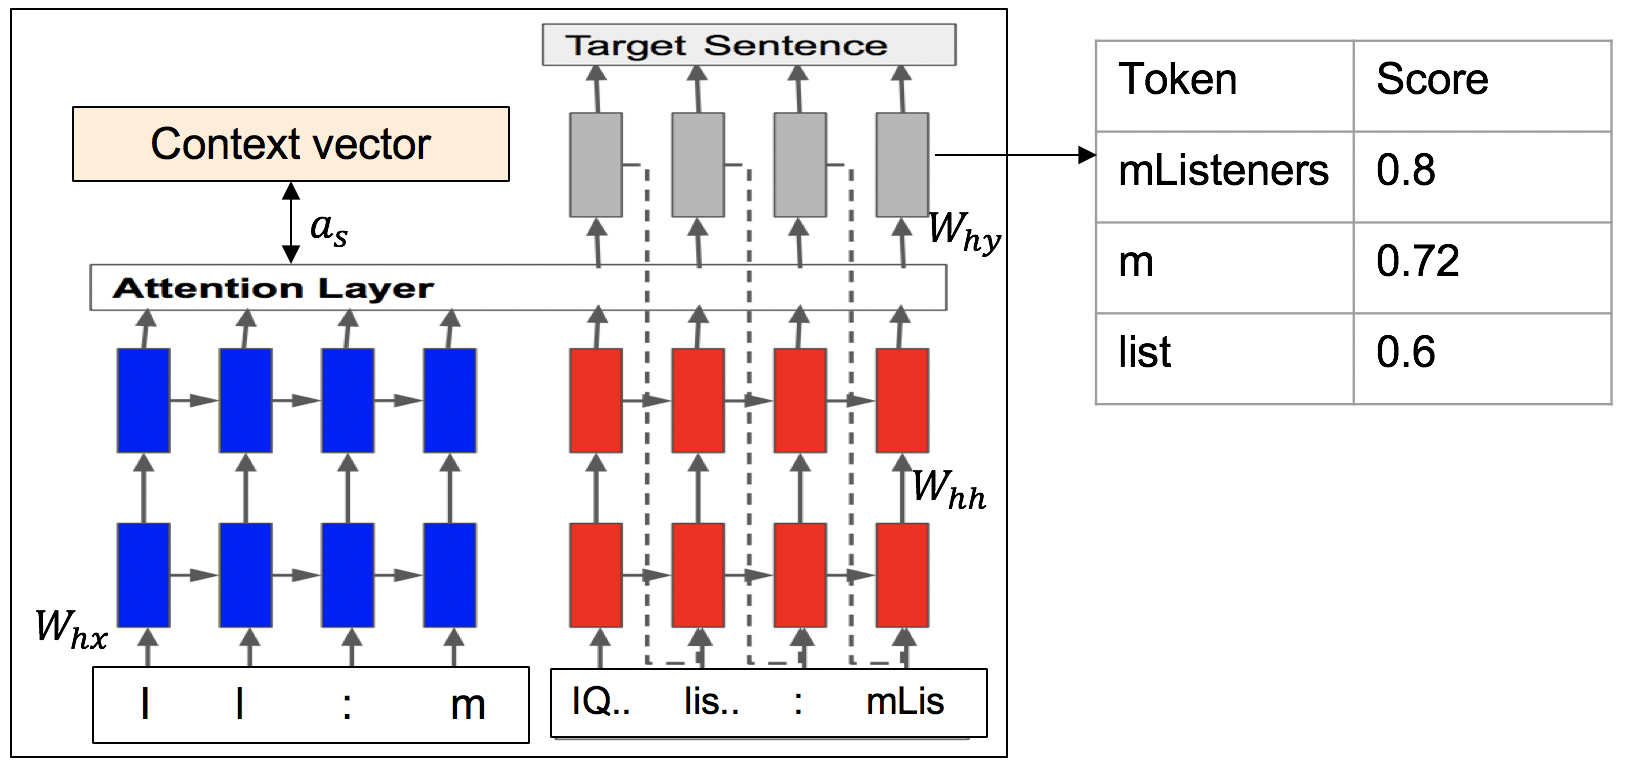
\includegraphics[width=\linewidth]
        {images/fig002.png}}
        \caption{NMT translation result of Listing \ref{example001}}
        \label{fig:002} 
\end{figure}

\textbf{Optimization of NMT for PrefixMap}. From formula \ref{eq:005}, we see that the NMT provides a distribution for all posible output, mean all possible tokens in the vocabulary. So that, it cannot work with too large vocabulary with more than 40000 words \cite{028}. To overcome this challenge, we replace the prefixes/ tokens with less than 10 times appearance as \textt{Unknown} token. We apply the same algorithm to reverse the order of the output of NMT like SMT model.  
\section{Evaluation}
We implement the tool PrefixMap with 2 Machine Translation engines.Since the idea of PrefixMap can also be applicable in different types of documents, we provide our experiment from all 3 types of documentations. They are Natural Language, Software Documentation and Programming Language. We also discuss on our results on comparing between Neural Machine Translation versus Statistical Machine Translation on this problem. We target to have the information about the prefix resolution based on different types of code tokens. In general, we want to answer the following research questions:

\begin{enumerate}
\item RQ1: Is prefix resolution important in programming language?
\item RQ2: Does NMT outperform SMT on PrefixMap by NLP translation evaluation metrics?
\item RQ3: Does NMT outperform SMT on PrefixMap by SE translation evaluation metrics?
\item RQ4: How SMT and NMT perform with different types of code prefixes?
\item RQ5: How SMT and NMT perform with ambiguous code prefixes?
\end{enumerate}

\subsection{Metrics for MT Evaluation}
We use 2 metrics reflect the view point of NLP and SE: the BLEU score and the exact matching accuracy. 
\\
\textbf{BLEU}. Bilingual Evaluation Understudy score, called the BLEU score, is the fundamental metric for comparing the actual output and expected output of the MT problem \cite{045}.  The BLEU score will take input as pair of expected and translated result, it will output as the score from 0 to 1 to reflect the similarity at n-gram level of word. The higher of BLEU, the better of translation engine performed. This score is calculated based on the co-occurrence at of n-gram between expected and translated sentence along with strategies for penalty and smoothing \cite{045}. We select the n-gram at 4-gram, and using the BLEU score implementation from Google NMT \cite{040}.

\textbf{Exact Match Accuracy}. In our MT problem, the requirement of good translation is not only restricted at the similar at n-gram. Similar to \cite{028}, another translation based approach in Software Engineering, we evaluate the Exact Match Accuracy at words level. Given the ith index of source sequence $prefix_{i}$ and of the expected sequence $expect_{i}$ and of the translated sequence $translate_{i}$, we compare the match between the $expect_{i}$ and $translate_{i}$. Since we have training data and testing data, we have Out of Vocabulary (OOV) cases. OOV has 2 types: Out of Source (OOS) means $prefix_{i}$ didn't appear in the training data and Out of Target (OOT) means $expect_{i}$ didn't exist in the training data. Since the prefix mapping process should suggest meaningful code token, we avoid evaluating the cases that the expected token was the same with prefix token. 

\subsection{Corpus Preparation}
We do the evaluation on 3 types of documentation:
\\
\textbf{Natural Language}. We collect all English sentences from the large scale corpus of English-German translation in NLP in \cite{040}. This corpus contains 1,15 millions sentences. 
\\
\textbf{Software Documentation}.We use the Conala corpus from \cite{046}. This corpus contains Python software documentation as 116000 English sentences.
\\
\textbf{Programming Language}.We collect 1000 Java projects from MSR 2013 corpus \cite{031}. We extract 560000 pairs of source and target tokens. The algorithm for extracting source and target language can be found in section 3.

For the variation of n-letter prefixes, we do the evaluation based on 3 levels: 1-letter prefix, 3-letters prefixes and 9-letters prefixes.




\subsection{MT Models Configurations}
Both SMT and NMT are run in a high end computer with Core i7 processor, 32 GB of RAM memory and using Nvidia RTX 2080 with 8GB of GPU.
\subsubsection{Statistical Machine Translation}
We use the default configuration suggested by Phrasal \cite{021}.The details of configuration is shown in \ref{tblConfigSMT}.
\begin{table}[]
\small
\centering
\begin{tabular}{|l|l|}
\hline
\textbf{Key }             & \textbf{Value} \\ \hline
MAX\_PHRASE\_LEN & 7     \\ \hline
Memory           & 26 GB \\ \hline
ttable-limit     & 250   \\ \hline
distortion-limit & 50    \\ \hline
stack            & 100   \\ \hline
\end{tabular}
\caption{Configuration of Statistical Machine Translation Model}
\label{tblConfigSMT}
\end{table}

\subsubsection{Neural Machine Translation}
Number of units in each hidden layer affects the accuracy \cite{047}. Increasing number of hidden unit can improve the accuracy but reduce the time performance since we need to change the batch size. So for NMT, we have 2 configurations as shown in Table \ref{tblConfigNMTs}.





\begin{table}[]
\small
\centering
\begin{tabular}{|l|l|l|}
\hline
\textbf{Key}                & \textbf{Config A (512 units)} & \textbf{Config B (1024 units)} \\ \hline
attention                   & normed\_bahdanau              & normed\_bahdanau               \\ \hline
attention\_architecture     & gnmt\_v2                      & gnmt\_v2                       \\ \hline
\textbf{batch\_size}        & \textbf{32}                   & \textbf{16}                    \\ \hline
beam\_width                 & 10                            & 10                             \\ \hline
decay\_scheme               & luong10                       & luong10                        \\ \hline
dropout                     & 0.2                           & 0.2                            \\ \hline
encoder\_type               & gnmt                          & gnmt                           \\ \hline
\textbf{infer\_batch\_size} & \textbf{32}                   & \textbf{16}                    \\ \hline
infer\_mode                 & greedy                        & greedy                         \\ \hline
init\_op                    & uniform                       & uniform                        \\ \hline
init\_weight                & 0.1                           & 0.1                            \\ \hline
learning\_rate              & 1                             & 1                              \\ \hline
length\_penalty\_weight     & 1                             & 1                              \\ \hline
num\_decoder\_layers        & 2                             & 2                              \\ \hline
num\_encoder\_layers        & 2                             & 2                              \\ \hline
\textbf{num\_train\_steps}         & \textbf{340000}                  & \textbf{680000} 
 \\ \hline
\textbf{num\_units}         & \textbf{512}                  & \textbf{1024} 
\\ \hline
optimizer                   & sgd                           & sgd                            \\ \hline
share\_vocab                & FALSE                         & FALSE                          \\ \hline
src\_max\_len               & 255                           & 255                            \\ \hline
steps\_per\_stats           & 100                           & 100                            \\ \hline
\end{tabular}
\caption{Configuration of Neural Machine Translation Models}
\label{tblConfigNMTs}
\end{table}



\subsection{Analysis on Length of Tokens in NL, SD and PL}
To answer RQ1, we analyze the average length of tokens in the target language of our NL, SD and PL corpus. The result is shown in Table \ref{tblAnalyzeOnPrefixLength}. By this table, we show that the average length of words in NL is over 6 letters in English. This is consistent with our hypothesis since we consider that NL usually intend to describe a single word in a token. Besides, the size of vocabulary in in NL corpus is around 20000, which is feasible for NMT to train and get the result without removing any unknown tokens.

For the SD and PL corpus, the result shows different characteristics of these data. For the average length, the PL corpus gains highest length of letter per separate words at over 16. THe PL also reveals a high average length of letters as over 11. This is the expected result, since in SD and PL, sentences are usually made by developers. Unlike NL, developers have to mention about AST elements such as method names and class names, which increases the number of letters per each tokens. This means the code completion tool that allows getting code from prefix is needed.

The other points from \ref{tblAnalyzeOnPrefixLength} also shows that the vocabulary size of each corpus are varied. In constrast to NL, the SD and PL corpus contains a remarkably bigger vocabulary. In our assumption, this fact is due to 2 reasons. First, the PL and SD contains tokens that mentioned several words. It means that they can be combination of tuple or triple of words instead of uni-word per token like NL. Secondly, the SD and PL can be developed by many developers with different code naming style, which cause many rare words appeared in the corpus.


\begin{table}[]
\small
\begin{tabular}{|l|l|l|}
\hline
\textbf{Target Languages}                                & \textbf{Vocab size}                                                    & \textbf{Average token length}                                                              \\ \hline
Natural Language                                & 19038                                                   & 6.08                                                              \\ \hline
Software Documentation                          & 134886                                                  & 11.77                                                             \\ \hline
Programming Language                            & 541275                                                  & 18.38                                                             \\ \hline
\end{tabular}
\caption{Analysis on Length of Tokens in NL, SD and PL}
\label{tblAnalyzeOnPrefixLength}
\end{table}

\subsection{BLEU Score Evaluation for Prefix Mapping NL, SD and PL}
In this experiment, we provide the translation for both NL, SD and PL corpus for SMT and configuration A of the SMT. The results are shown in Table \ref{tblBLEUScoreNLSDPL} and Table \ref{tblBLEUScoreConfigAAndB}. Along with these experiments, we have a verification experiment, which we run the configuration A on the English-German translation by \cite{040}. We got the accuracy of BLEU score at \textbf{29.74} compared to \textbf{29.9} of Google NMT, which shows the validity of our NMT configurations. For NL SD, we use 1-letter prefix as the source language.

From Table \ref{tblBLEUScoreNLSDPL}, we show that the increasing of BLEU score from NL, SD to PL. The NL has the lowest BLEU score. The reason is that we are doing the mapping from a context of 26 letters in NL to the target tokens which contains 19000 words, which caused challenges for the MT models. The PL corpus at 1-letter prefix returns surprisingly higher BLEU score. It shows the potential of capturing the code tokens based on code context can be better than in NL and SD. The BLEU score increases if we change the length of the prefixes.

We talk about the comparison between MT models. We got the accuracy of SMT outperforms the NMT with all of the corpus. This fact shows the strength of SMT to resolve the characteristic of consistent order between source and target language. We have a comparison of BLEU score between configuration A and B. It shows that the accuracy in configuration B increases, which shows the important of increasing number of hidden units.




\begin{table}[]
\small
\begin{tabular}{|l|l|l|}
\hline
\multicolumn{1}{|c|}{\textbf{Problems}}   & \multicolumn{1}{c|}{\textbf{SMT}} & \multicolumn{1}{c|}{\textbf{NMT (config A)}} \\ \hline
Natural Language                          & 13.36                             & 8.67                                         \\ \hline
Software Documentation                    & 53.11                             & 24.09                                        \\ \hline
Programming Language (1-letter prefixes)  & 63.4                              & 53.99                                        \\ \hline
Programming Language (5-letters prefixes) & 84.9                              & 64.33                                        \\ \hline
Programming Language (9-letters prefixes) & 92.61                             & 74.42                                        \\ \hline
\end{tabular}
\caption{BLEU Score Evaluation using SMT and NMT in NL, SD and PL}
\label{tblBLEUScoreNLSDPL}
\end{table}

\begin{table*}[]
\small
\begin{tabular}{|l|l|l|}
\hline
\multicolumn{1}{|c|}{\textbf{Problems}}   & \multicolumn{1}{c|}{\textbf{NMT (Config A)}} & \multicolumn{1}{c|}{\textbf{NMT (Config B)}} \\ \hline
Programming Language (1-letter prefixes)  & 53.99                                        & 52.78                                        \\ \hline
Programming Language (5-letters prefixes) & 64.33                                        & 73.39                                        \\ \hline
Programming Language (9-letters prefixes) & 74.42                                        & 79.12                                        \\ \hline
\end{tabular}
\caption{BLEU Score Comparison between Config A and B of NMT}
\label{tblBLEUScoreConfigAAndB}
\end{table*}


\subsection{Exact Match Accuracy Comparison of Prefix Mapping in NL, SD and PL}
The exact match accuracy are shown in Table \ref{tblExactMatchAccuracySMTAndNMT} and Table \ref{tblExactMatchAccuracyNMTConfigB}. From these tables, we show the accuracy of the prefix resolution varied depending on the types of n-letters prefixes. First, we see that we don't have the OOS case in the NL, SD and PL. This makes sense since the fact that we have a vocabulary of less than 100 prefixes in the source language of these configuration. However, with the SMT, we achieve over \textbf{65\%} of precision score, showing the strength of SMT in this type of problem. For 9-letter prefixes, the accuracy gained to \textbf{90\%}, means if developers wrote 9 letters of the code token, there are 9 per 10 cases the tool suggested correctly. We didn't include the non-useful suggestions counted to this accuracy. In the other words, the expected tokens need to be longer in letter than the prefixes.

For the NMT, the result is lower remarkably for Config A but improve in Config B. We got the accuracy ranged from 61\% from 1-letter prefix to 74\% for 9-letters prefixes for configuration A of NMT. For configuration B, the precision ranked from 58.62\% to 82.55\%. Though the gap between configuration B and SMT is only 8\%, the other problem of the NMT is the OOV tokens. For 9-prefixes letter, we got the OOV of NMT as high as third times the OOV of SMT. This is caused by the fact that there is a set of words required to change to Unknown words, which can badly impact the total accuracy of NMT.


\begin{table*}[]
\small
\begin{tabular}{|l|l|l|l|l|l|l|l|l|}
\hline
\textbf{Problems}                         & \multicolumn{8}{c|}{\textbf{SMT}}                                                                                                       \\ \hline
\textbf{}                                 & \textbf{Correct} & \textbf{Incorrect} & \textbf{OOS} & \textbf{OOT} & \textbf{OOV} & \textbf{Precision} & \textbf{Recall} & \textbf{F1} \\ \hline
Natural Language                          & 12671            & 35890              & 0            & 196          & 196          & 26.09\%            & 98.48\%         & 41.25\%     \\ \hline
Software Documentation                    & 40656            & 20176              & 0            & 1855         & 1855         & 66.83\%            & 95.64\%         & 78.68\%     \\ \hline
PL (1-letter prefixes)  & 53868            & 28529              & 0            & 4090         & 4090         & 65.38\%            & 92.94\%         & 76.76\%     \\ \hline
PL (5-letters prefixes) & 40164            & 7897               & 540          & 3337         & 3877         & 83.57\%            & 91.20\%         & 87.22\%     \\ \hline
PL (9-letters prefixes) & 20554            & 2207               & 1374         & 1753         & 3127         & 90.30\%            & 86.80\%         & 88.51\%     \\ \hline
                                          & \multicolumn{8}{c|}{\textbf{NMT (Config A)}}                                                                                            \\ \hline
\textbf{}                                 & \textbf{Correct} & \textbf{Incorrect} & \textbf{OOS} & \textbf{OOT} & \textbf{OOV} & \textbf{Precision} & \textbf{Recall} & \textbf{F1} \\ \hline
Natural Language                          & 10487            & 38074              & 0            & 196          & 196          & 21.60\%            & 98.17\%         & 35.40\%     \\ \hline
Software Documentation                    & 26237            & 31700              & 0            & 4750         & 4750         & 45.29\%            & 84.67\%         & 59.01\%     \\ \hline
PL (1-letter prefixes)  & 44510            & 28711              & 0            & 13266        & 13266        & 60.79\%            & 77.04\%         & 67.96\%     \\ \hline
PL (5-letters prefixes) & 25565            & 13895              & 3758         & 8720         & 12478        & 64.79\%            & 67.20\%         & 65.97\%     \\ \hline
PL (9-letters prefixes) & 11778            & 4217               & 7263         & 2630         & 9893         & 73.64\%            & 54.35\%         & 62.54\%     \\ \hline
\end{tabular}
\caption{Exact Match Accuracy Comparison between SMT and NMT Config A}
\label{tblExactMatchAccuracySMTAndNMT}
\end{table*}


\begin{table*}[]
\small
\begin{tabular}{|l|l|l|l|l|l|l|l|l|}
\hline
\multicolumn{1}{|c|}{\textbf{Problems}}             & \multicolumn{8}{c|}{\textbf{NMT (Config B)}}                               \\ \hline
                                                    & Correct & Incorrect & OOS  & OOT   & OOV   & Precision & Recall  & F1      \\ \hline
PL (1-letter prefixes)  & 42919   & 30302     & 0    & 13266 & 13266 & 58.62\%   & 76.39\% & 66.33\% \\ \hline
PL (5-letter prefixes) & 30853   & 8607      & 3758 & 8720  & 12478 & 78.19\%   & 71.20\% & 74.53\% \\ \hline
PL (9-letter prefixes) & 13204   & 2791      & 7263 & 2630  & 9893  & 82.55\%   & 57.17\% & 67.55\% \\ \hline
\end{tabular}
\caption{Exact Match Accuracy Comparison of NMT model Config B}
\label{tblExactMatchAccuracyNMTConfigB}
\end{table*}

\subsection{Analysis on Types of Tokens in Naming Conventions for Prefixes}
To setup this experiment, we provide a module that check the regular expression of each tokens in the testing data set. There are regular expressions on checking if a numeric, a class name, a variable, a method name or a string literal. We found and add the regular expressions for checking at well-known online resource as \cite{048,049}. Considering the Configuration B as a higher accuracy NMT model compared to configuration A. The results are shown in Table \ref{tblAnaTypeTokensSMT} and Table \ref{tblAnaTypeTokensNeuralMT}.

The result shows the consistent between NMT and SMT configuration. The two types of token received lowest accuracy is Numeric and String literal. The numeric tokens got precision as 34\% in 1-letter prefix of SMT and got 24.71\% in 1-letter prefix of NMT configuration B. The String literal got 28\% in each configuration. This fact reveals the challenge of code suggestion for numeric and string literal, since the they are not only depend on the tokens but also depend on the control flow or data flow graph of the program. For main types of tokens, we got the highest accuracy for class name while the variable name and constanct tokens achieved the equal results in both SMT and NMT. It is explainable since the good class names can be reused popular by developers which helps the SMT model to learn the prediction. Method name, in the other hands, varied based on the purpose of each developers.

\begin{table}[]
\tiny
\begin{tabular}{|l|l|l|l|l|l|l|l|l|}
\hline
\multicolumn{9}{|c|}{\textbf{SMT (1-letter prefixes)}}                                        \\ \hline
Type of Tokens     & Correct & Incorrect & OOS  & OOT  & OOV  & Precision & Recall  & F1      \\ \hline
Total:             & 53868   & 28529     & 0    & 4090 & 4090 & 65.38\%   & 92.94\% & 76.76\% \\ \hline
NumericType:       & 163     & 304       & 0    & 28   & 28   & 34.90\%   & 85.34\% & 49.54\% \\ \hline
ClassNameType:     & 6154    & 2793      & 0    & 317  & 317  & 68.78\%   & 95.10\% & 79.83\% \\ \hline
VariableType:      & 26937   & 14888     & 0    & 1503 & 1503 & 64.40\%   & 94.72\% & 76.67\% \\ \hline
MethodNameType:    & 12908   & 6695      & 0    & 501  & 501  & 65.85\%   & 96.26\% & 78.20\% \\ \hline
StringLiteralType: & 628     & 1585      & 0    & 841  & 841  & 28.38\%   & 42.75\% & 34.11\% \\ \hline
ConstanctType:     & 1321    & 821       & 0    & 281  & 281  & 61.67\%   & 82.46\% & 70.57\% \\ \hline
OtherType:         & 5757    & 1443      & 0    & 619  & 619  & 79.96\%   & 90.29\% & 84.81\% \\ \hline
\multicolumn{9}{|c|}{\textbf{SMT (5-letter prefixes)}}                                        \\ \hline
Total:             & 40164   & 7897      & 540  & 3337 & 3877 & 83.57\%   & 91.20\% & 87.22\% \\ \hline
NumericType:       & 81      & 65        & 7    & 12   & 19   & 55.48\%   & 81.00\% & 65.85\% \\ \hline
ClassNameType:     & 6986    & 755       & 40   & 270  & 310  & 90.25\%   & 95.75\% & 92.92\% \\ \hline
VariableType:      & 17271   & 3861      & 258  & 1096 & 1354 & 81.73\%   & 92.73\% & 86.88\% \\ \hline
MethodNameType:    & 10924   & 2057      & 23   & 474  & 497  & 84.15\%   & 95.65\% & 89.53\% \\ \hline
StringLiteralType: & 1219    & 389       & 100  & 730  & 830  & 75.81\%   & 59.49\% & 66.67\% \\ \hline
ConstanctType:     & 1182    & 404       & 29   & 243  & 272  & 74.53\%   & 81.29\% & 77.76\% \\ \hline
OtherType:         & 2501    & 366       & 83   & 512  & 595  & 87.23\%   & 80.78\% & 83.88\% \\ \hline
\multicolumn{9}{|c|}{\textbf{SMT (9-letter prefixes)}}                                        \\ \hline
Total:             & 20554   & 2207      & 1374 & 1753 & 3127 & 90.30\%   & 86.80\% & 88.51\% \\ \hline
NumericType:       & 11      & 3         & 2    & 0    & 2    & 78.57\%   & 84.62\% & 81.48\% \\ \hline
ClassNameType:     & 4279    & 233       & 116  & 160  & 276  & 94.84\%   & 93.94\% & 94.39\% \\ \hline
VariableType:      & 6436    & 950       & 511  & 431  & 942  & 87.14\%   & 87.23\% & 87.19\% \\ \hline
MethodNameType:    & 6963    & 557       & 185  & 279  & 464  & 92.59\%   & 93.75\% & 93.17\% \\ \hline
StringLiteralType: & 868     & 179       & 288  & 456  & 744  & 82.90\%   & 53.85\% & 65.29\% \\ \hline
ConstanctType:     & 923     & 155       & 104  & 114  & 218  & 85.62\%   & 80.89\% & 83.19\% \\ \hline
OtherType:         & 1074    & 130       & 168  & 313  & 481  & 89.20\%   & 69.07\% & 77.85\% \\ \hline
\end{tabular}
\caption{Analysis Result on Types of Tokens for Prefix Mapping by SMT}
\label{tblAnaTypeTokensSMT}
\end{table}

\begin{table*}[]
\small
\begin{tabular}{|l|l|l|l|l|l|l|l|l|}
\hline
\multicolumn{9}{|c|}{\textbf{NMT in Config B (1-letter prefixes)}}                                                                                                \\ \hline
\textbf{Type of Tokens} & \textbf{Correct} & \textbf{Incorrect} & \textbf{OOS} & \textbf{OOT} & \textbf{OOV} & \textbf{Precision} & \textbf{Recall} & \textbf{F1} \\ \hline
Total:                  & 42919            & 30302              & 0            & 13266        & 13266        & 58.62\%            & 76.39\%         & 66.33\%     \\ \hline
NumericType:            & 86               & 262                & 0            & 147          & 147          & 24.71\%            & 36.91\%         & 29.60\%     \\ \hline
ClassNameType:          & 4554             & 3343               & 0            & 1367         & 1367         & 57.67\%            & 76.91\%         & 65.91\%     \\ \hline
VariableType:           & 21774            & 16366              & 0            & 5188         & 5188         & 57.09\%            & 80.76\%         & 66.89\%     \\ \hline
MethodNameType:         & 10742            & 7065               & 0            & 2297         & 2297         & 60.32\%            & 82.38\%         & 69.65\%     \\ \hline
StringLiteralType:      & 354              & 902                & 0            & 1798         & 1798         & 28.18\%            & 16.45\%         & 20.77\%     \\ \hline
ConstanctType:          & 875              & 586                & 0            & 962          & 962          & 59.89\%            & 47.63\%         & 53.06\%     \\ \hline
OtherType:              & 4534             & 1778               & 0            & 1507         & 1507         & 71.83\%            & 75.05\%         & 73.41\%     \\ \hline
\multicolumn{9}{|c|}{\textbf{NMT in Config B (5-letters prefixes)}}                                                                                               \\ \hline
Total:                  & 30853            & 8607               & 3758         & 8720         & 12478        & 78.19\%            & 71.20\%         & 74.53\%     \\ \hline
NumericType:            & 40               & 18                 & 84           & 23           & 107          & 68.97\%            & 27.21\%         & 39.02\%     \\ \hline
ClassNameType:          & 5473             & 1245               & 444          & 889          & 1333         & 81.47\%            & 80.41\%         & 80.94\%     \\ \hline
VariableType:           & 13575            & 4153               & 1402         & 3356         & 4758         & 76.57\%            & 74.05\%         & 75.29\%     \\ \hline
MethodNameType:         & 8843             & 2366               & 227          & 2042         & 2269         & 78.89\%            & 79.58\%         & 79.23\%     \\ \hline
StringLiteralType:      & 512              & 202                & 862          & 862          & 1724         & 71.71\%            & 22.90\%         & 34.71\%     \\ \hline
ConstanctType:          & 727              & 223                & 305          & 603          & 908          & 76.53\%            & 44.46\%         & 56.25\%     \\ \hline
OtherType:              & 1683             & 400                & 434          & 945          & 1379         & 80.80\%            & 54.96\%         & 65.42\%     \\ \hline
\multicolumn{9}{|c|}{\textbf{NMT in Config B (9-letters prefixes)}}                                                                                               \\ \hline
Total:                  & 13204            & 2791               & 7263         & 2630         & 9893         & 82.55\%            & 57.17\%         & 67.55\%     \\ \hline
NumericType:            & 6                & 3                  & 6            & 1            & 7            & 66.67\%            & 46.15\%         & 54.55\%     \\ \hline
ClassNameType:          & 3082             & 580                & 827          & 299          & 1126         & 84.16\%            & 73.24\%         & 78.32\%     \\ \hline
VariableType:           & 3632             & 1244               & 2645         & 807          & 3452         & 74.49\%            & 51.27\%         & 60.74\%     \\ \hline
MethodNameType:         & 5254             & 673                & 1335         & 722          & 2057         & 88.65\%            & 71.86\%         & 79.38\%     \\ \hline
StringLiteralType:      & 251              & 75                 & 1168         & 297          & 1465         & 76.99\%            & 14.63\%         & 24.58\%     \\ \hline
ConstanctType:          & 456              & 91                 & 632          & 117          & 749          & 83.36\%            & 37.84\%         & 52.05\%     \\ \hline
OtherType:              & 523              & 125                & 650          & 387          & 1037         & 80.71\%            & 33.53\%         & 47.37\%     \\ \hline
\end{tabular}
\caption{Analysis Result on Types of Tokens for Prefix Mapping by NMT}
\label{tblAnaTypeTokensNeuralMT}
\end{table*}

\subsection{Analysis on the Accuracy of PrefixMap on Ambiguous Tokens}
In the last experiment, we analyze the affect of the number of mapping prefixes to code tokens can affect the accuracy. For each prefix in the training set, we run a program to check how many distinct code tokens are mapped to that prefix in the target language. The prefix that has more mapped tokens can be considered as more ambiguous. The result can be shown in Table \ref{tblAnaPercentageMappingSMT} for SMT and Table \ref{tblAnaPercentageMappingNeuralMT} for NMT configuration B.

The first observation we got is that in 1-letter prefix, there is no case of mapping 1-1 to tokens in both SMT and NMT. This fact is explainable since the vocabulary of the source language contains only letters in alphabet and number digits, which are less than 100 prefixes. Besides, there are a large percentage of the prefixes has more than 100 mappings with 1-letter prefix corpus. For the 1-letter prefix, the SMT got accuracy about 70\% while the NMT got 59\% for very ambiguous tokens. For 5-letters and 9-letter prefixes, the accuracy of SMT decreases from unambiguous tokens to very ambiguous tokens. In the NMT with 9-letters prefix and for very ambiguous tokens, these tokens are considered as Unknown due to their rarely appeared in the data set, cause the NMT to decrease. In general, the SMT outperforms the NMT for almost all of accuracy experiments.


\begin{table}[]
\tiny
\begin{tabular}{|l|l|l|l|l|l|l|}
\hline
\multicolumn{7}{|c|}{\textbf{SMT (1-letter prefixes)}}                                                           \\ \hline
TokenType\textbackslash{}NumofMap & 1         & 2-10      & 11-20     & 21-50     & 51-100    & Greater than 100 \\ \hline
                                  & Precision & Precision & Precision & Precision & Precision & Precision        \\ \hline
NumericType:                      & 0.00\%    & 0.00\%    & 0.00\%    & 0.00\%    & 0.00\%    & 34.90\%          \\ \hline
ClassNameType:                    & 0.00\%    & 0.00\%    & 0.00\%    & 0.00\%    & 0.00\%    & 68.78\%          \\ \hline
VariableType:                     & 0.00\%    & 0.00\%    & 0.00\%    & 100.00\%  & 0.00\%    & 64.40\%          \\ \hline
MethodNameType:                   & 0.00\%    & 0.00\%    & 0.00\%    & 0.00\%    & 0.00\%    & 65.85\%          \\ \hline
StringLiteralType:                & 0.00\%    & 0.00\%    & 0.00\%    & 0.00\%    & 0.00\%    & 28.38\%          \\ \hline
ConstanctType:                    & 0.00\%    & 0.00\%    & 0.00\%    & 0.00\%    & 0.00\%    & 61.67\%          \\ \hline
OtherType:                        & 0.00\%    & 40.00\%   & 97.35\%   & 83.18\%   & 0.00\%    & 70.68\%          \\ \hline
Total of tokens:                  & 0         & 10        & 2416      & 221       & 1         & 79749            \\ \hline
Percentage:                       & 0.00\%    & 0.01\%    & 2.93\%    & 0.27\%    & 0.00\%    & 96.79\%          \\ \hline
\multicolumn{7}{|c|}{\textbf{SMT (5-letter prefixes)}}                                                           \\ \hline
NumericType:                      & 100.00\%  & 57.78\%   & 71.43\%   & 36.84\%   & 60.00\%   & 0.00\%           \\ \hline
ClassNameType:                    & 100.00\%  & 91.83\%   & 88.90\%   & 87.06\%   & 90.34\%   & 89.09\%          \\ \hline
VariableType:                     & 100.00\%  & 80.09\%   & 78.40\%   & 77.36\%   & 82.91\%   & 81.70\%          \\ \hline
MethodNameType:                   & 100.00\%  & 94.60\%   & 89.77\%   & 90.62\%   & 89.03\%   & 80.35\%          \\ \hline
StringLiteralType:                & 100.00\%  & 85.04\%   & 75.63\%   & 74.70\%   & 68.45\%   & 65.50\%          \\ \hline
ConstanctType:                    & 100.00\%  & 83.66\%   & 79.35\%   & 75.09\%   & 66.67\%   & 58.60\%          \\ \hline
OtherType:                        & 100.00\%  & 87.09\%   & 84.58\%   & 90.91\%   & 91.85\%   & 82.38\%          \\ \hline
Total of tokens:                  & 1980      & 6425      & 3375      & 6411      & 7017      & 22853            \\ \hline
Percentage:                       & 4.12\%    & 13.37\%   & 7.02\%    & 13.34\%   & 14.60\%   & 47.55\%          \\ \hline
\multicolumn{7}{|c|}{\textbf{SMT (9-letter prefixes)}}                                                           \\ \hline
NumericType:                      & 100.00\%  & 100.00\%  & 50.00\%   & 75.00\%   & 0.00\%    & 0.00\%           \\ \hline
ClassNameType:                    & 100.00\%  & 94.22\%   & 90.73\%   & 89.12\%   & 89.56\%   & 83.10\%          \\ \hline
VariableType:                     & 100.00\%  & 84.45\%   & 77.86\%   & 72.23\%   & 74.80\%   & 57.25\%          \\ \hline
MethodNameType:                   & 100.00\%  & 92.64\%   & 87.54\%   & 91.82\%   & 85.10\%   & 80.07\%          \\ \hline
StringLiteralType:                & 100.00\%  & 84.38\%   & 69.66\%   & 68.29\%   & 71.74\%   & 59.85\%          \\ \hline
ConstanctType:                    & 100.00\%  & 80.74\%   & 66.27\%   & 72.46\%   & 64.71\%   & 66.67\%          \\ \hline
OtherType:                        & 100.00\%  & 88.58\%   & 81.52\%   & 90.79\%   & 88.46\%   & 53.33\%          \\ \hline
Total of tokens:                  & 6360      & 9952      & 1808      & 2550      & 1302      & 789              \\ \hline
Percentage:                       & 27.94\%   & 43.72\%   & 7.94\%    & 11.20\%   & 5.72\%    & 3.47\%           \\ \hline
\end{tabular}
\caption{Analysis Result on How PrefixMapping can handle Ambiguous Tokens by SMT}
\label{tblAnaPercentageMappingSMT}
\end{table}

\begin{table*}[]
\small
\begin{tabular}{|l|l|l|l|l|l|l|}
\hline
\multicolumn{7}{|c|}{\textbf{NMT in Config B (1-letter prefixes)}}                                                                                                              \\ \hline
\textbf{TokenType\textbackslash{}NumofMap} & \textbf{1}         & \textbf{2-10}      & \textbf{11-20}     & \textbf{21-50}     & \textbf{51-100}    & \textbf{\textgreater 100} \\ \hline
                                           & \textbf{Precision} & \textbf{Precision} & \textbf{Precision} & \textbf{Precision} & \textbf{Precision} & \textbf{Precision}        \\ \hline
NumericType:                               & 0.00\%             & 0.00\%             & 66.67\%            & 29.79\%            & 30.77\%            & 23.16\%                   \\ \hline
ClassNameType:                             & 0.00\%             & 0.00\%             & 25.00\%            & 62.50\%            & 0.00\%             & 57.68\%                   \\ \hline
VariableType:                              & 0.00\%             & 0.00\%             & 0.00\%             & 0.00\%             & 19.64\%            & 57.15\%                   \\ \hline
MethodNameType:                            & 0.00\%             & 0.00\%             & 0.00\%             & 0.00\%             & 50.00\%            & 60.33\%                   \\ \hline
StringLiteralType:                         & 0.00\%             & 0.00\%             & 0.00\%             & 0.00\%             & 0.00\%             & 28.18\%                   \\ \hline
ConstanctType:                             & 0.00\%             & 0.00\%             & 66.67\%            & 0.00\%             & 0.00\%             & 59.96\%                   \\ \hline
OtherType:                                 & 0.00\%             & 89.25\%            & 50.00\%            & 66.29\%            & 35.29\%            & 58.76\%                   \\ \hline
Total:                                     & 0                  & 2661               & 32                 & 324                & 90                 & 70114                     \\ \hline
Percentage:                                & 0.00\%             & 3.63\%             & 0.04\%             & 0.44\%             & 0.12\%             & 95.76\%                   \\ \hline
\multicolumn{7}{|c|}{\textbf{NMT in Config B (5-letters prefixes)}}                                                                                                             \\ \hline
NumericType:                               & 76.47\%            & 66.67\%            & 64.29\%            & 0.00\%             & 0.00\%             & 0.00\%                    \\ \hline
ClassNameType:                             & 79.67\%            & 84.24\%            & 79.10\%            & 76.19\%            & 84.81\%            & 0.00\%                    \\ \hline
VariableType:                              & 70.64\%            & 74.03\%            & 78.03\%            & 85.35\%            & 64.47\%            & 57.97\%                   \\ \hline
MethodNameType:                            & 91.36\%            & 88.80\%            & 82.14\%            & 81.87\%            & 74.68\%            & 63.74\%                   \\ \hline
StringLiteralType:                         & 75.74\%            & 67.24\%            & 77.88\%            & 70.83\%            & 0.00\%             & 0.00\%                    \\ \hline
ConstanctType:                             & 87.64\%            & 76.84\%            & 75.58\%            & 47.73\%            & 53.42\%            & 0.00\%                    \\ \hline
OtherType:                                 & 92.73\%            & 75.98\%            & 73.26\%            & 88.68\%            & 77.80\%            & 83.33\%                   \\ \hline
Total:                                     & 3324               & 10580              & 6002               & 10938              & 5283               & 3333                      \\ \hline
Percentage:                                & 8.42\%             & 26.81\%            & 15.21\%            & 27.72\%            & 13.39\%            & 8.45\%                    \\ \hline
\multicolumn{7}{|c|}{\textbf{NMT in Config B (9-letters prefixes)}}                                                                                                             \\ \hline
NumericType:                               & 0.00\%             & 66.67\%            & 0.00\%             & 0.00\%             & 0.00\%             & 0.00\%                    \\ \hline
ClassNameType:                             & 83.72\%            & 86.38\%            & 76.40\%            & 68.18\%            & 0.00\%             & 0.00\%                    \\ \hline
VariableType:                              & 77.08\%            & 72.33\%            & 70.32\%            & 68.24\%            & 0.00\%             & 0.00\%                    \\ \hline
MethodNameType:                            & 92.88\%            & 88.57\%            & 80.41\%            & 67.58\%            & 77.50\%            & 0.00\%                    \\ \hline
StringLiteralType:                         & 78.17\%            & 71.43\%            & 87.10\%            & 0.00\%             & 0.00\%             & 0.00\%                    \\ \hline
ConstanctType:                             & 88.08\%            & 73.86\%            & 50.00\%            & 0.00\%             & 0.00\%             & 0.00\%                    \\ \hline
OtherType:                                 & 73.49\%            & 78.28\%            & 91.72\%            & 66.67\%            & 0.00\%             & 0.00\%                    \\ \hline
Total:                                     & 7403               & 6748               & 1300               & 504                & 40                 & 0                         \\ \hline
Percentage:                                & 46.28\%            & 42.19\%            & 8.13\%             & 3.15\%             & 0.25\%             & 0.00\%                    \\ \hline
\end{tabular}
\caption{Analysis Result on How PrefixMapping can handle Ambiguous Tokens by NMT}
\label{tblAnaPercentageMappingNeuralMT}
\end{table*}


\section*{Related Works}

The characteristics of our parallel corpus appeared in other SE problems \cite{027,028}. In these works, SMT outperforms NMT in accuracy. In general, SE researches have specific characteristics of corpus, which brings rooms for deep learning and machine learning to  improve their approaches. Other researches show drawbacks of Machine Learning in SE. \cite{050} and point out the drawbacks of machine learning approach for method name recommendation that is usually suggest too simple method names. \cite{022} shows that the original SMT has problems of exponential time increasing with big data. For the code suggestion area, other research works focuses on a specific types of code tokens. \cite{051} suggested method name based on Hierachical Attention Networks, and \cite{052} suggested method name and class name. In our work, we intend to generate all types of tokens based on writing the abbreviations or prefixes. 


\section*{Conclusion}
In this work, we propose PrefixMap, a code suggestion tool for all types of code tokens in Java programming language. To realize our idea, we propose two Machine Translation models, Statistical Machine Translation and Neural Machine Translation, which learn the information from source language as the space of abbreviation or prefix to the target language as actual code tokens. Our work shows that we got an accuracy from 60\% to 90\% for SMT and from 59\% to 83\% for NMT. In the Machine Learning point of view, we reveal a class of parallel corpus which SMT can learn more information and get better accuracy on NMT in Software Engineering. Two of the characteristics of SE parallel corpus are the unknown tokens problem and being consistent on the length and the order of the source and target corpus. 

There are a few limitations of our work. First, the space of all prefixes are rarely happened in the practice. Secondly, we use a very simple approach to treat the unknown token for NMT. As future work, we will study how abbreviations are written by developers to support more types of abbreviation suggestions instead of suggesting only by prefix, and apply optimization of NMT in other area such as \cite{023} to improve the accuracy. The data is available at \cite{053}.

\clearpage

\bibliographystyle{plainurl}
\bibliography{refs}


\end{document}
